\chapter{Redes de distribuição de conteúdo}
%\section{Composi\c{c}\~ao de uma \emph{Content Delivery Network}} 
\label{sec:composicao}

Para entendermos melhor uma Redes de distribuição de conteúdo (\emph{Content Delivery Network} - CDN), precisamos primeiro destrich\'a-la em v\'arios pequenos peda\c{c}os para assim compreendê-la em uma maneira global.

Uma CDN apesar de ,abstratamente, ser vista como um mecanismo \'unico, pode ser vista tamb\'em como a soma de v\'arios tipos de elementos e caracter\'isticas que somadas e configuradas formar\'a um mecanismo \'unico e transparente aos usu\'arios.

Fazem parte dessas caracter\'isticas: organiza\c{c}\~ao, tipos de servidores, protocolos e tipos de conte\'udo. Que serão detalhados nesse capítulo.

\section{Visão Geral}

\textcolor{red}{Generalizar CDNs em um paragrafo - Citar exemplos como Netflix, spotify e até serviços de noticias do android}

Quanto a organiza\c{c}\~ao uma CDN pode ser uma rede unicamente CDN ou uma rede \textit{overlay}, que nada mais \'e que uma rede onde ela tenta abstrai as camadas de redes j\'a existentes(como transporte, redes entre outras) e transforma-l\'a em uma rede puramente CDN.

Os tipos de conte\'udo que ir\~ao ser transportados dentro da rede s\~ao fundamentais para definir diversos aspectos de configura\c{c}\~oes que ser\~ao utilizadas dentro da rede. Como por exemplo, a forma de Cache que ser\~ao feitas os arquivos ou at\'e mesmo a forma como v\~ao ser distribu\'idos, se ser\~ao distribu\'idos em conjunto ou em partes. 

\section{Tipos de servidores}
\label{section:tipos_de_servidores}
Há dois tipos servidores: Servidor de origem e servidor de ponta. Isso independente de suas configurações físicas(quantidade de memória, CPU, HD e \emph{etc}).

\subsection{Servidores de origem}

S\~ao servidores de origem servidores onde toda a informa\c{c}\~ao que irá ser consumida fica baseado. \'E o lugar onde os conte\'udos v\~ao ser primeiramente armazenados e/ou gerados e é o ponto principal do sistema.

\'E ele o respons\'avel por, na aus\^encia da informa\c{c}\~ao perto do cliente, fornecer tudo o que o cliente necessita de informa\c{c}\~ao. Normalmente em primeiros acessos.

H\'a uma necessidade intr\'inseca de que esse servidor tenha excelentes configura\c{c}\~oes f\'isicas e \'otimas regras de seguran\c{c}as, \textit{firewall} a principal delas, que possam garantir a integridade do sistema mesmo em caso de muitos acessos.

\subsection{Servidores de ponta}
S\~ao servidores que mais pr\'oximos aos clientes. Parte do conte\'udo do servidor de origem estar\'a replicado nele. Dizemos em parte, pois n\~ao sabemos quais pol\'iticas de \textit{cache} que ser\'a adotada pelos criadores da rede. 
\\
Podemos ilustr\'a-los conforme a figura \ref{figura:tipos_servidores}.
\begin{figure}[H]
\caption{Tipos de servidores}
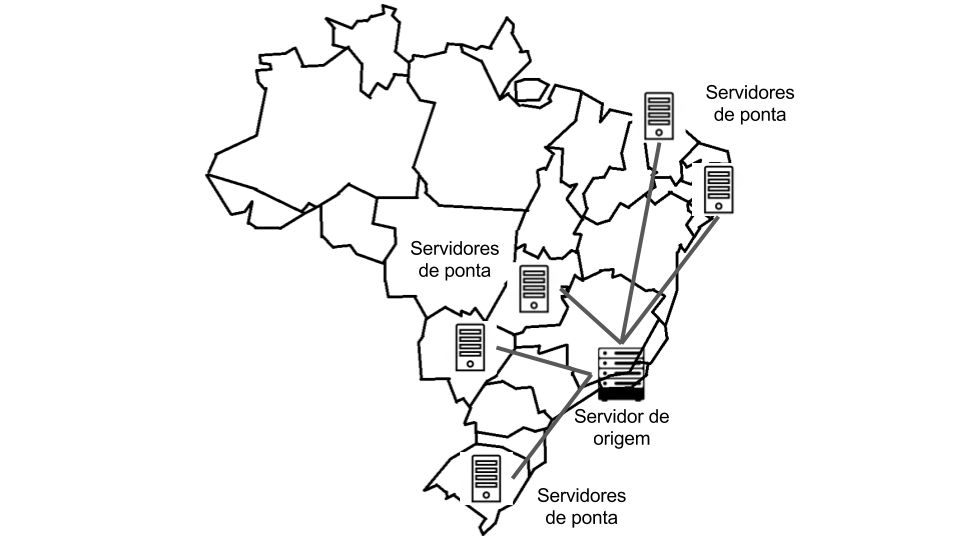
\includegraphics[height=9cm]{Figuras/tipos_servidores.png} 
\label{figura:tipos_servidores} 
\end{figure}

Vale salientar que esses \textit{status} de ser de ponta ou ser de origem não s\~ao imut\'aveis. Em ambientes reais e comerciais um servidor de origem \'e tamb\'em um servidor de ponta para um outro conte\'udo. Isso \'e o respons\'avel por tornar as grandes \emph{CDNs} completamente transparentes geograficamente perante aos seus clientes.
\section{Protocolos de intera\c{c}\~oes}
\label{section:protocolos_interacoes}
\begin{figure}[H]
\caption{Tipos de relacionamentos}
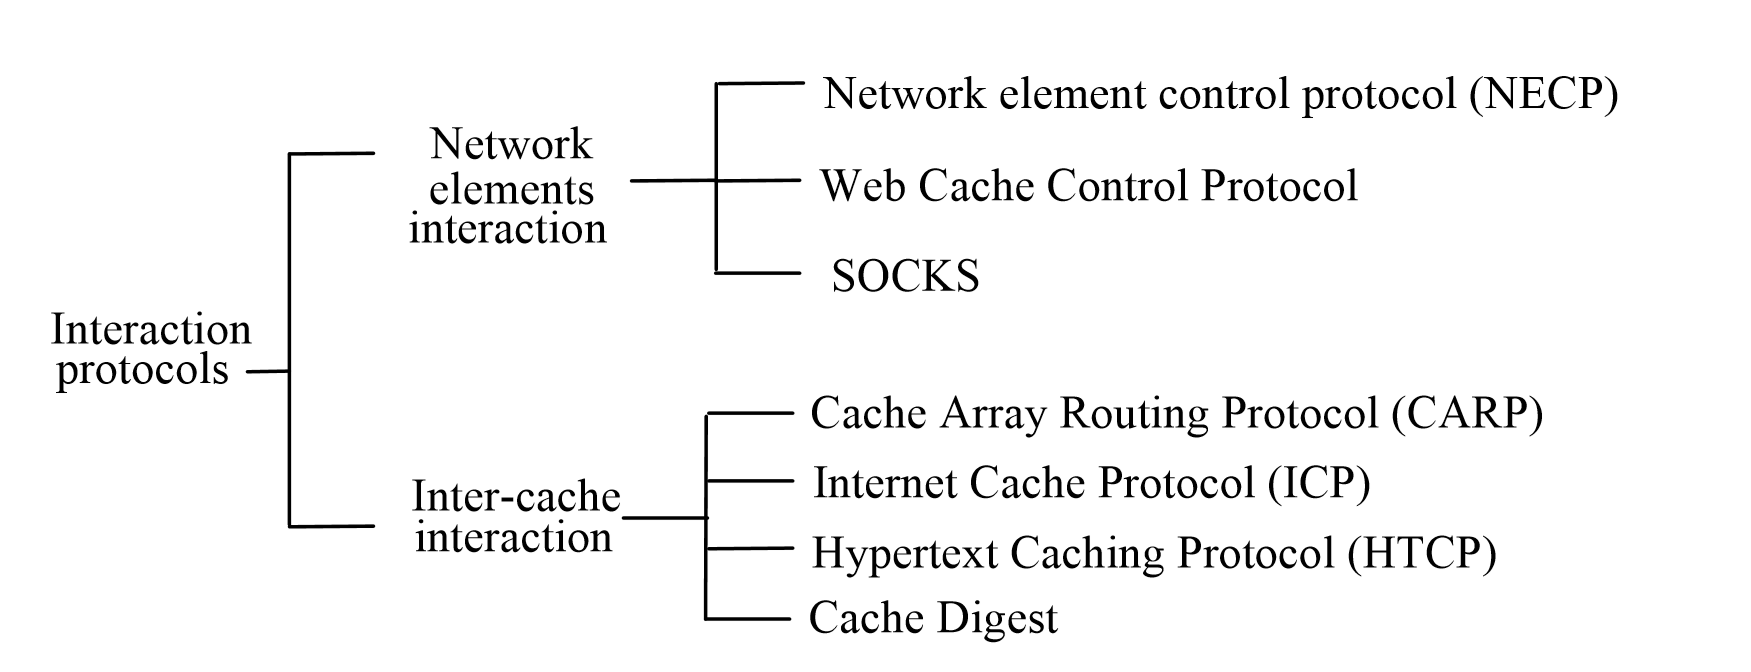
\includegraphics[width=15cm]{Figuras/tipos_relacionamentos.png} 
\label{figura:tipos_relacionamentos}
\end{figure}

Os protocolos de intera\c{c}\~oes podem ser divididos em duas partes: Protocolos de intera\c{c}\~oes de elementos da rede e Protocolos de intera\c{c}\~oes entre os servidores de cache da CDN. 


\subsection{Intera\c{c}\~oes dos elementos da rede}
\begin{figure}[H]
\caption{Tipos de protocolos de itera\c{c}\~oes}
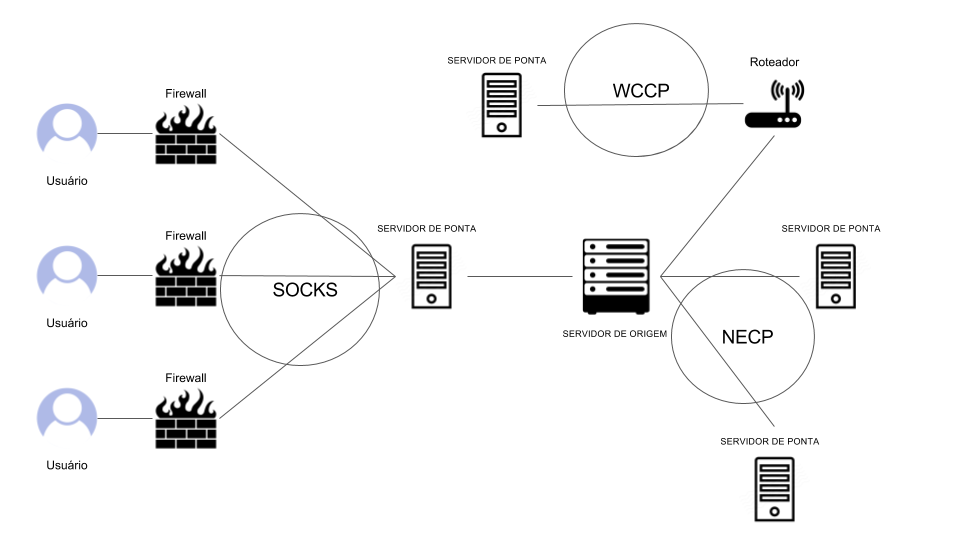
\includegraphics[height=9cm]{Figuras/protocolos_interacao_elementos.png} 
\label{figura:protocolos_interacao_elementos}
\end{figure}

Dentro dos protocolos de intera\c{c}\~oes dos elementos de rede podemos verificar que cada um possui sua especificidade e funcionalidade bem definida, como podemos ver na figura \ref{figura:protocolos_interacao_elementos} , tentando proteger n\~ao s\'o a rede mas tamb\'em o usu\'ario, o servidor, os roteadores e a comunica\c{c}\~ao entre os mesmos.
\paragraph{Socks} \'e um protocolo desenhado para um \textit{framework} para aplica\c{c}\~oes cliente-servidor que rodem em TCP ou UDP e utilizem os servi{c}os do \textit{firewall}. Sua principal funcionalidade \'e gerar um t\'unel de comunica\c{c}\~ao seguro entre cliente e servidor.
\paragraph{NECP} \'e um protocolo leve de comunica\c{c}\~ao que serve para sinalizar o tr\'afico entre os elementos da rede.
\paragraph{WCCP} serve para itera\c{c}\~oes entre roteadores e \textit{web-caches}	e tamb\'em para transporte entre os mesmos.


\subsection{Intera\c{c}\~oes de cache}

Os protocolos de intera\c{c}\~oes de cache s\~ao protocolos que organizam as trocas de informa\c{c}\~oes entre os servidores, ou seja, \'e ele que dita como ir\'a funcionar a distribui\c{c}\~ao da informa\c{c}\~ao dentro da rede.
 Conforme vimos na figura \ref{figura:tipos_relacionamentos}, e segundo \cite{pathan2007taxonomy}, existem 4 tipos de protocolos aplicados nessa circunst\^ancia como podemos ver na figura \ref{figura:protocolos_interacao_cache}
\begin{figure}[H]
\caption{Tipos de protocolos de itera\c{c}\~oes}
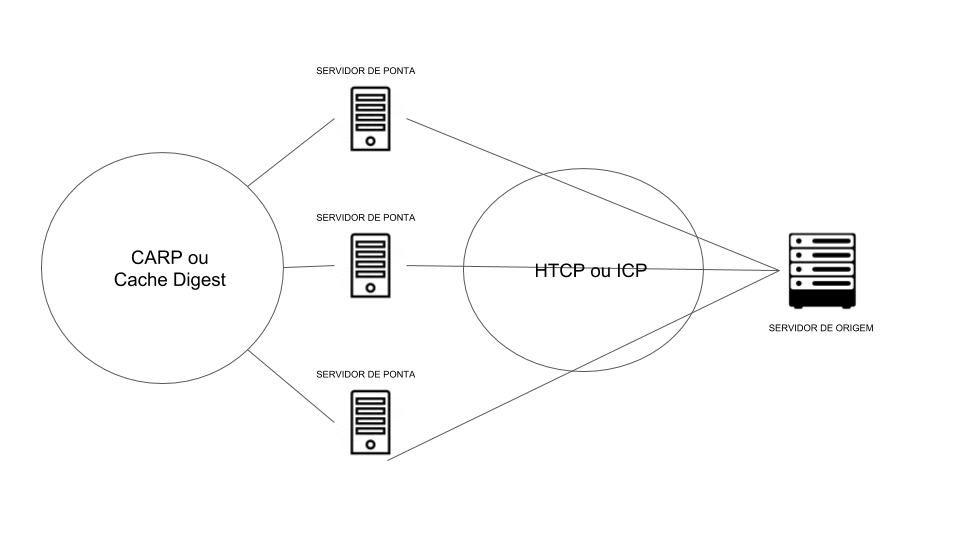
\includegraphics[height=9cm]{Figuras/protocolos_interacoes_cache.png} 
\label{figura:protocolos_interacao_cache}
\end{figure}

Dois deles s\~ao: HTCP - Hypertext Caching Protocol e ICP - Internet Cache Protocol que s\~ao concorrentes entre s\'i e tem como funcionalidade controlar o fluxo de informa\c{c}\~ao entre os caches. Sendo atrav\'es deles que se controla o que ir\'a para um determinado servidor de ponta, por exemplo. Falaremos mais sobre ambos em \ref{section:HTCP} e \ref{section:ICP} respectivamente.
 Existe tamb\'em os protocolos CARP -  Cache Array Routing Protocol e Cache Digest, tamb\'em concorrentes, servem para controlar o conte\'udo existente dentro de cada servidor e saber onde est\~ao os outros conte\'udos. Falaremos mais sobre ambos em \ref{section:CARP} e \ref{section:Cache Digest} respectivamente.

\subsection{HTCP}
\label{section:HTCP}
Como dito anteriormente o HTCP, Hypertext Caching Protocol, \'e um protocolo de intera\c{c}\~ao entre os caches, suas principais caracterist\'icas s\~ao:
\begin{itemize}
\item Protocolo para descobrir Caches HTTP;
\item Suporte ao HTTP 1.0;
\item Permite incluir cabeçalhos nas respostas;
\item Podem ser enviados via TCP/UDP;
\item Devem ser resilientes a falhas.
\end{itemize}

\subsection{ICP}
\label{section:ICP}
J\'a o ICP, Internet Cache Protocol, \'e um protocolo muito mais leve que possui as seguintes caracterist\'icas:
\begin{itemize}
\item Protocolo de mensagem leve;
\item Utilizado para comunica\c{c}\~ao de Caches;
\item Utiliza consultas para determinar localiza\c{c}\~ao mais apropriada;
\item Suporte ao HTTP 0.9;
\item Comunica-se com caches vizinhos;
\item recebe MISS ou HIT como resposta;
\item Enviado via UDP;
\item Falha por timeout indica caminho quebrado;
\item Fornece informa\c{c}\~oes para balanceamento atrav\'es das medidas de perda.
\end{itemize}

\subsection{HTCP x ICP}
Analisando os dois protocolos HTCP e ICP, podemos fazer um quadro comparativo entre eles e coloc\'a-los da seguinte maneira(figura \ref{figura:htcp_x_icp}):

\begin{figure}[H]
\caption{HTCP x ICP}
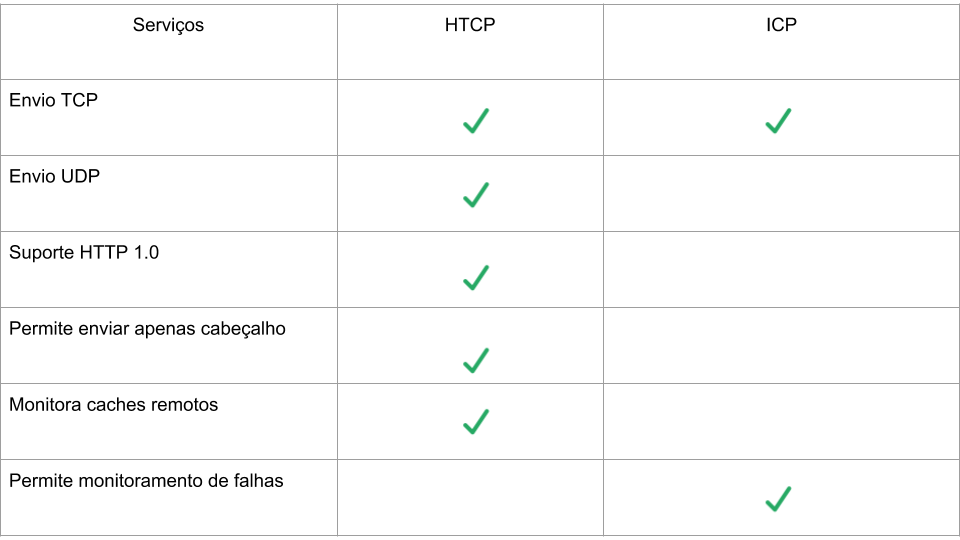
\includegraphics[height=9cm]{Figuras/htcp_x_icp.png} 
\label{figura:htcp_x_icp}
\end{figure}

\subsection{CARP}
\label{section:CARP}
CARP -  Cache Array Routing Protocol
 Protocolo de armazenamento distribu\'ido baseado em uma lista conhecida de proxies fracamente acoplada e uma fun\c{c}\~ao hash para dividir o espa\c{c}o URL entre esses proxies.
\begin{itemize}
\item Cliente HTTP pode enviar requisi\c{c}\~ao \`a qualquer proxy da lista.
\end{itemize}

\subsection{Cache Digest}
\label{section:Cache Digest}
Protocolo de interc\^ambio e formato de dados entre caches.
\begin{itemize}
\item Fornece um resumo dos conte\'udos na resposta;
\item Soluciona os problemas de congestionamento e timeout;
\item Torna poss\'ivel determinar se um servidor possui em cache um conte\'udo;
\item Executado via HTTP ou FTP;
\item Cont\'em tempo de expira\c{c}\~ao na resposta;
\item Pode ser utilizados para eliminar redund\^ancia.
\end{itemize}

\section{Sele\c{c}\~ao e entrega de conte\'udo}
\label{section:selecaoentrega}
Dentro de uma CDN temos que  nos preocupar com a forma como esse conte\'udo vai catalogado, armazenado e distribu\'ido dentro da rede, o que vimos no item \ref{section:protocolos_interacoes}, como tamb\'em temos que nos preocupar como esse conte\'udo vai chegar at\'e o cliente (usu\'ario) da forma mais otimizada poss\'ivel, ou seja, o servidor o qual vai fornecer as informa\c{c}\~oes para ele ser\'a o mais perto ou mais r\'apido. 
 Temos que destacar tamb\'em a import\^ancia da otimiza\c{c}\~ao do fluxo de informa\c{c}\~ao pela rede. Visto que quanto maior o tr\'afico de informa\c{c}\~ao pela rede significa que a informa\c{c}\~ao est\'a mais distante do usu\'ario e tamb\'em que vai ter um custo maior pela troca intensa de informa\c{c}\~ao. 
 Segundo \cite{krishnamurthy2001use}, na tentativa de otimizar o redirecionamentos de URL para o usu\'ario se sacramentou dois tipos de t\'ecnicas de redirecionamentos, Full - site e Partial - site.

\subsection{Full - site}
Na t\'ecnica de Full-site todo o conte\'udo \'e entregado ao usu\'ario de um servidor ponta \'unico. Ou seja, o usu\'ario faz uma requisi\c{c}\~ao ao servidor principal, onde o mesmo processa um algoritmo de roteamento para encontrar o servidor ponta que melhor se enquadra como resposta, e ent\~ao retorna ao usu\'ario o endere\c{c}o onde ent\~ao ser\'a consumido por fim todas as informa\c{c}\~oes requisitadas. 
 \'E importante salientar que essa t\'ecnica \'e amplamente utilizada por servi\c{c}os que fazem pouco uso de dados da rede. Uma p\'agina est\'atica da web, por exemplo, se encaixaria perfeitamente nesse contexto. Visto que possui baixo grau de modifica\c{c}\~oes e seu tamanho \'e pequeno perto de outros tipos de m\'idias que circulam na web.

\subsection{Partial - site}
J\'a redirecionamentos do tipo Partial-sites os servidores principais retornam para o usu\'ario uma parte do conte\'udo e disparam, automaticamente, um algoritmo de roteamento para encontrar o restante da informa\c{c}\~ao e retornar ao usu\'ario. Conforme podemos ver na figura \ref{figura:entrega_conteudo}
\begin{figure}[H]
\caption{Entrega de conte\'udo}
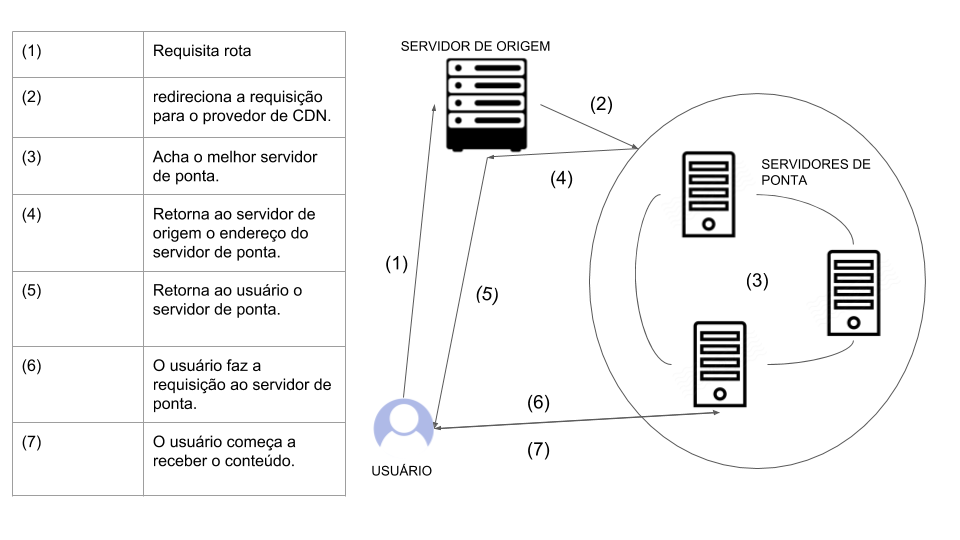
\includegraphics[height=9cm]{Figuras/entrega_conteudo.png} 
\label{figura:entrega_conteudo}
\end{figure}
Nela podemos ver que todo o processo acontece em basicamente sete etapas. (1) o usu\'ario faz uma requisi\c{c}\~ao ao servidor principal onde este dispara (2) um roteamento (3) para buscar qual \'e o melhor servidor para aquele usu\'ario. Depois, em (4) o servidor principal recebe a identifica\c{c}\~ao do servidor de ponta e repassa ao usu\'ario (5) juntamente com um arquivo que cont\'em as informa\c{c}\~oes centrais que normalmente s\~ao iguais para o mundo todo. Em seguida o usu\'ario come\c{c}a a enviar (6) e receber (7) informa\c{c}\~oes com o servidor de ponta.

 Entretanto h\'a em (3) diversas formas de fazer esse roteamento quanto a distribui\c{c}\~ao do conte\'udo pela rede e quanto a aglomera\c{c}\~ao desse conte\'udo dentro do servidores de cache. 
 Tipo de distribui\c{c}\~ao nada mais \'e do que a forma como o conte\'udo vai ser disperso na rede, como esse conte\'udo vai se aproximar do n\'o que est\'a mais perto do usu\'ario. 

Os tipos de distribui\c{c}\~ao mais frequentemente utilizados s\~ao o emp\'irico e o por popularidade.

Emp\'irico trata, como o pr\'oprio nome diz, de uma forma de distribui\c{c}\~ao sem nenhum conhecimento espec\'ifico a respeito, utilizando-se apenas um conhecimento experimental de onde seria melhor posicionado o conte\'udo.
 Em um esquema baseado em popularidade a distribui\c{c}\~ao \'e feita conforme a notoriedade. Ou seja, quanto maior o n\'umero de requisi\c{c}\~oes a um conte\'udo, mais ele ser\'a distribu\'ido nos servidores de ponta perto do usu\'ario.
 Ambos esquemas n\~ao s\~ao necessariamente excludentes, pode-se inicialmente aplicar a forma empir\'ica para gerar dados a respeito da distribui\c{c}\~ao e depois utilizar esses dados para aplicar o modo de popularidade.
	
Tamb\'em existe as formas de aglomera\c{c}\~oes de conte\'udo. Isso existe porque os conte\'udos podem ser conjuntos de objetos ou objetos independentes. 
As formas de aglomera\c{c}\~oes s\~ao por objeto e por conjunto de objetos.

Aglomera\c{c}\~ao por objeto vai juntar os objetos mais selecionados e distribu\'i-los individualmente entre os servidores. J\'a por conjunto de objetos ele vai separ\'a-los em grupos e distribui-los em conjuntos. 
 Podemos exemplicar da seguinte forma: Em um site temos v\'arios elementos, temos o HTML, temos o CSS e temos a m\'idia de um v\'ideo qualquer. Podemos separar da seguinte forma: temos 3 elementos onde 2 deles s\~ao altamente dependentes(HTML e CSS) e temos 1 que pode ser diferente em cada regi\~ao do pa\'is, que \'e o v\'ideo. 
 Ent\~ao podemos misturar as formas de aglomera\c{c}\~oes. Para o HTML e para o CSS agrupamos em conjuntos de objetos; e para o v\'ideo fazemos a aglomera\c{c}\~ao por objeto,j\'a que ser\'a distribu\'ido de maneira independente nos servidores.

Analisando os tipos,perceber-se que nenhuma das op\c{c}\~oes s\~ao excludentes entre s\'i, pode-se combinar quaisquer tipo de distribui\c{c}\~ao e aglomera\c{c}\~ao e as escolhas v\~ao depender das necessidades de cada aplica\c{c}\~ao.\'E necess\'ario uma an\'alise minuciosa de cada aplica\c{c}\~ao para chegar em um veredito da melhor abordagem.
\subsection{VOD}
\label{subsec:vod}
\paragraph{VOD - Video on Demand} - Segundo \cite{garfinkle1996video}, \'e um sistema de que proporciona uma interface de comunica\c{c}\~ao com o usu\'ario de produtos dispon\'iveis de uma esta\c{c}\~ao central remota.
 \'E um sistema muito utilizado por operadoras de conte\'udo onde \'e o cliente quem decide o hor\'ario que ir\'a consumir determinado conte\'udo.
 Isso permite \`as pessoas que tinham que esperar o hor\'ario certo para consumir determinado conte\'udo, poderem a qualquer momento e em qualquer lugar fazer uso do mesmo.
\paragraph{Microsoft Smooth Streaming} \'E um sistema de consumo de v\'ideo onde a qualidade do v\'ideo transmitida vai ser definida conforme a qualidade da banda dispon\'ivel. Clientes que possuem alta disponibilidade de banda ter\~ao maior qualidade do v\'ideo. 
 Para conseguir tocar um v\'ideo nesse formato o player do usu\'ario tem que ser capaz de interpretar um manifesto que cont\'em dentro de outras coisas, o caminho de onde est\'a localizado a m\'idia desejada. 
 J\'a para conseguir fazer a transi\c{c}\~ao de qualidade o v\'ideo \'e quebrado em pequenos peda\c{c}os chamados de "chunks". Ent\~ao, conforme \'e verificada um aumento ou decremento da banda dispon\'ivel o player come\c{c}ar que consumir chunks de qualidade diferente da atual alternando assim o \textit{bitrate} do v\'ideo que est\'a sendo consumido. 
 No artigo \cite{zambelli2009iis} podemos ver todas as aplica\c{c}\~oes e implica\c{c}\~oes dessa forma de consumo de m\'idia.
\subsection{VOD na pr\'atica}
\label{subsubsection:vod_exemplo}
Agora vamos ilustrar com um exemplo mais pr\'atico. Utilizaremos uma requisi\c{c}\~ao de uma URL de um VOD (Video On Demand) onde a parte de roteamento \'e feita no usu\'ario. A aplica\c{c}\~ao do usu\'ario faz uma requisi\c{c}\~ao \`a CDN e enquanto o cabe\c{c}alho da resposta n\~ao for 200 ele vai ler um campo dentro do cabe\c{c}alho de resposta e fazer uma nova requisi\c{c}\~ao. A figura  \ref{figura:vod_redirect_exemple} ilustra a situa\c{c}\~ao.

\begin{figure}[H]
\caption{Redirecionamento de CDN}
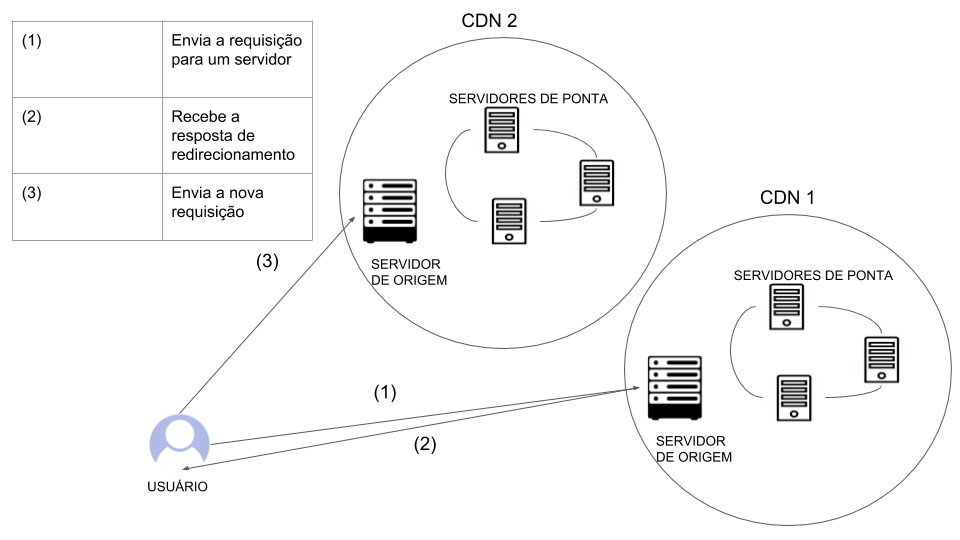
\includegraphics[width=15cm]{Figuras/vod_redirect_exemple.png} 
\label{figura:vod_redirect_exemple}
\end{figure}

\section{Considerações Finais}

Redes CDNs apesar de serem quase transparentes aos usuários não signfica que são simples. Como vimos possuem diversas características que devem ser levadas em consideração ao serem montadas ou estudadas. Em cada característica dessa é possível desenvolver diversos tipos de pesquisas.

Nesse trabalho iremos focar somente na entrega do conteúdo desejado (\ref{section:selecaoentrega}). Especificamente quanto a entrega de conteúdo de VOD (\ref{subsubsection:vod_exemplo}).